\documentclass[a4paper,11pt]{article}

\usepackage{préambule}

\TitreDActivite{Activité : Introduction à Scratch}

\begin{document}

\maketitle

\begin{greybox}[frametitle={Pour commencer}]
	Pour lancer Scratch : cliquer sur le menu, puis rechercher 'scratch'. Lancer le programme 'Scratch 2'.

	\includegraphics[width=\textwidth]{Images/panneau scratch 2 - annoté.jpg}

	\begin{enumerate}
		\item Pour changer la langue.
		\item Panneau des \textbf{blocks}.

		      Certains blocks on des zones dans lesquelles on peut écrire, comme 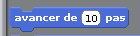
\includegraphics[width=5em]{Images/Block avancer de 10 pas.png}.
		\item Panneau des \textbf{scripts}.
		\item Bouton 'démarrer' et 'stop'.
	\end{enumerate}
\end{greybox}

\begin{exercice}
	Pour lancer un programme, il \myuline{faut} utiliser un block de \textit{Contrôle}, en jaune. Place le block drapeau (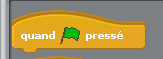
\includegraphics[width=5em]{Images/Block drapeau.png}) dans le panneau des scripts. \\

	Puis, expérimente avec les block d'\textit{Apparence} violets : place en 1 ou plus sous le block drapeau, et décrit ce qu'il se passe :
	\begin{itemize}
		\item Quel est l'effet du block \squared{Dire Salut!} ? Que se passe-t-il si on met un block \squared{Dire Salut!} suivi de \squared{Dire Bonjour!} ? \vspace{0.5em}

		      \dotfill
		\item Quel est l'effet du block \squared{modifier la taille par 10} ? Essayer en remplaçant le nombre par 20, puis par 100. \vspace{0.5em}

		      \dotfill
		\item Quel est l'effet du block \squared{mettre la taille à 100\%} ? Essayer en remplaçant le nombre par 200, puis par 50. \vspace{0.5em}

		      \dotfill
	\end{itemize}
\end{exercice}

\newpage

\begin{exercice}[: Variables]
	Dans la catégorie \textit{Variables}, clique sur “Nouvelle variable”. Donne le nom “nombre” à cette nouvelle variable.

	De nouveau blocks apparaissent : ils permettent de manipuler ce nouvel objet qu'on vient de créer, “nombre”.

	Crée un programme contenant :
	\begin{itemize}
		\item Un block drapeau
		\item Un block \squared{à nombre attribuer 0}
		\item Un block 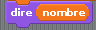
\includegraphics[width=3em]{Images/Dire nombre.png}. Pour créer ce block, il faut placer un block \squared{Dire Salut!}, puis faire glisser le block “nombre” sur “Salut!”.
	\end{itemize}

	Sans le lancer, peux-tu dire ce que va faire ce programme ? \vspace{0.5em}

	\dotfill\vspace{0.5em}

	\dotfill

	\begin{greybox}
		Une variable, comme son nom l'indique, peut \textbf{varier}.
	\end{greybox}

	En combinant les blocks déjà vus, fais en sorte que le personnage dise “0”, puis “1”. Utilise le block jaune \squared{Attendre 1 seconde} pour qu'on puisse voir le changement.
\end{exercice}

\begin{exercice}[: Boucles]
	Grâce au blocks de \textit{Contrôle} jaunes, on peut faire en sorte qu'une action soit effectuée plusieurs fois de suite. \vspace{1em}

	Utilise ces blocks pour faire dire au personnage tous les nombres entiers (Indice : on pourra utiliser le block \squared{changer nombre par 1}).
\end{exercice}

\begin{exercice*}[Bonus: trouve le nombre]
	Dans \textit{Capteurs}, on peut trouver de quoi demander à l'utilisateur de rentrer un nombre.

	Utilise cette fonctionnalité pour implémenter un jeu de \textbf{trouve le nombre} :
	\begin{itemize}
		\item l'utilisateur rentre un nombre.
		\item Si c'est le nombre à deviner, on dit “Trouvé !”.
		\item Si le nombre est trop petit, on dit “Trop petit !”, et on redemande un nombre.
		\item Si le nombre est trop grand, on dit “Trop grand !”, et on redemande un nombre.
	\end{itemize}
\end{exercice*}

\end{document}